\documentclass[conference]{IEEEtran}
% Some/most Computer Society conferences require the compsoc mode option,
% but others may want the standard conference format.


% *** CITATION PACKAGES ***
% 
\ifCLASSOPTIONcompsoc
% IEEE Computer Society needs nocompress option
% requires cite.sty v4.0 or later (November 2003)
\usepackage[nocompress]{cite}
\else
% normal IEEE
\usepackage{cite}
\fi
% cite.sty was written by Donald Arseneau
% V1.6 and later of IEEEtran pre-defines the format of the cite.sty package
% \cite{} output to follow that of the IEEE. Loading the cite package will
% result in citation numbers being automatically sorted and properly
% "compressed/ranged". e.g., [1], [9], [2], [7], [5], [6] without using
% cite.sty will become [1], [2], [5]--[7], [9] using cite.sty. cite.sty's
% \cite will automatically add leading space, if needed. Use cite.sty's
% noadjust option (cite.sty V3.8 and later) if you want to turn this off
% such as if a citation ever needs to be enclosed in parenthesis.
% cite.sty is already installed on most LaTeX systems. Be sure and use
% version 5.0 (2009-03-20) and later if using hyperref.sty.
% The latest version can be obtained at:
% http://www.ctan.org/pkg/cite
% The documentation is contained in the cite.sty file itself.
% 
% Note that some packages require special options to format as the Computer
% Society requires. In particular, Computer Society  papers do not use
% compressed citation ranges as is done in typical IEEE papers
% (e.g., [1]-[4]). Instead, they list every citation separately in order
% (e.g., [1], [2], [3], [4]). To get the latter we need to load the cite
% package with the nocompress option which is supported by cite.sty v4.0
% and later.




\usepackage[pdftex]{graphicx}
\graphicspath{{./png/}}
\DeclareGraphicsExtensions{.pdf,.jpeg,.png}

% *** GRAPHICS RELATED PACKAGES ***
% 
\ifCLASSINFOpdf
% \usepackage[pdftex]{graphicx}
% declare the path(s) where your graphic files are
% \graphicspath{{../pdf/}{../jpeg/}}
% and their extensions so you won't have to specify these with
% every instance of \includegraphics
%\DeclareGraphicsExtensions{.pdf,.jpeg,.png}
\else
% or other class option (dvipsone, dvipdf, if not using dvips). graphicx
% will default to the driver specified in the system graphics.cfg if no
% driver is specified.
% \usepackage[dvips]{graphicx}
% declare the path(s) where your graphic files are
% \graphicspath{{../eps/}}
% and their extensions so you won't have to specify these with
% every instance of \includegraphics
% \DeclareGraphicsExtensions{.eps}
\fi
% graphicx was written by David Carlisle and Sebastian Rahtz. It is
% required if you want graphics, photos, etc. graphicx.sty is already
% installed on most LaTeX systems. The latest version and documentation
% can be obtained at: 
% http://www.ctan.org/pkg/graphicx
% Another good source of documentation is "Using Imported Graphics in
% LaTeX2e" by Keith Reckdahl which can be found at:
% http://www.ctan.org/pkg/epslatex
% 
% latex, and pdflatex in dvi mode, support graphics in encapsulated
% postscript (.eps) format. pdflatex in pdf mode supports graphics
% in .pdf, .jpeg, .png and .mps (metapost) formats. Users should ensure
% that all non-photo figures use a vector format (.eps, .pdf, .mps) and
% not a bitmapped formats (.jpeg, .png). The IEEE frowns on bitmapped formats
% which can result in "jaggedy"/blurry rendering of lines and letters as
% well as large increases in file sizes.
% 
% You can find documentation about the pdfTeX application at:
% http://www.tug.org/applications/pdftex


% *** MATH PACKAGES ***
\usepackage{amsmath}
\interdisplaylinepenalty=2500

% *** SPECIALIZED LIST PACKAGES ***
% 
% \usepackage{algorithmic}
% algorithmic.sty was written by Peter Williams and Rogerio Brito.
% This package provides an algorithmic environment fo describing algorithms.
% You can use the algorithmic environment in-text or within a figure
% environment to provide for a floating algorithm. Do NOT use the algorithm
% floating environment provided by algorithm.sty (by the same authors) or
% algorithm2e.sty (by Christophe Fiorio) as the IEEE does not use dedicated
% algorithm float types and packages that provide these will not provide
% correct IEEE style captions. The latest version and documentation of
% algorithmic.sty can be obtained at:
% http://www.ctan.org/pkg/algorithms
% Also of interest may be the (relatively newer and more customizable)
% algorithmicx.sty package by Szasz Janos:
% http://www.ctan.org/pkg/algorithmicx




% *** ALIGNMENT PACKAGES ***
% 
% \usepackage{array}
% Frank Mittelbach's and David Carlisle's array.sty patches and improves
% the standard LaTeX2e array and tabular environments to provide better
% appearance and additional user controls. As the default LaTeX2e table
% generation code is lacking to the point of almost being broken with
% respect to the quality of the end results, all users are strongly
% advised to use an enhanced (at the very least that provided by array.sty)
% set of table tools. array.sty is already installed on most systems. The
% latest version and documentation can be obtained at:
% http://www.ctan.org/pkg/array

\hyphenation{op-tical net-works semi-conduc-tor}

\begin{document}
\title{A Proposal for an Intuitionistic Fuzzy Inference System}


\author{\IEEEauthorblockN{Amaury Hernandez-Aguila, Mario
    Garcia-Valdez, Oscar Castillo}
  \IEEEauthorblockA{Tijuana Institute of Technology\\
    Division of Graduate Studies and Graduates\\
    Tijuana, Mexico\\
    Email: \{amherag,mario,ocastillo\}@tectijuana.edu.mx}}

\maketitle

\begin{abstract}

\end{abstract}

\IEEEpeerreviewmaketitle



\section{Introduction}



\section{Related Work}

\section{Preliminaries}

% intuitionistic fuzzy set
\begin{equation}
  A^{*} = \{\langle x, \mu _{A} (x), \nu _{A} (x) \rangle | x \in E\}
\end{equation}

% intuitionistic interval
\begin{equation}
  0 \leq \mu_{A}(x) + \nu_{A}(x) \leq 1
\end{equation}

% every ordinary fuzzy set has the form
\begin{equation}
  \{ \langle x, \mu_{A}(x), 1 - \mu_{A}(x) \rangle | x \in E \}
\end{equation}

% if
\begin{equation}
  \pi_{A}(x) = 1 - \mu_{A}(x) - \nu_{A}(x)
\end{equation}

\section{Proposed Method}

\begin{enumerate}
  \item if $t_{0}$ is $A_{1}$ then $p_{t+1}$ is $C_{1}$
  \item if $t_{-6}$ is $A_{2}$ then $p_{t+1}$ is $C_{2}$
  \item if $t_{-12}$ is $A_{3}$ then $p_{t+1}$ is $C_{3}$
  \item if $t_{-18}$ is $A_{4}$ then $p_{t+1}$ is $C_{4}$
\end{enumerate}

\begin{figure}[!t]
  \centering
  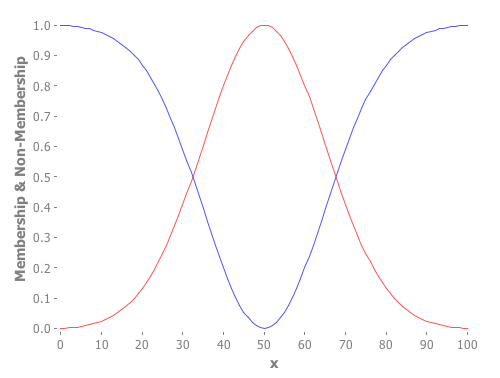
\includegraphics[width=2.5in]{fs-as-ifs}
  \caption{Classic Fuzzy Set Represented as an Intuitionistic Fuzzy Set}
  \label{fs-as-ifs}
\end{figure}

\begin{figure}[!t]
  \centering
  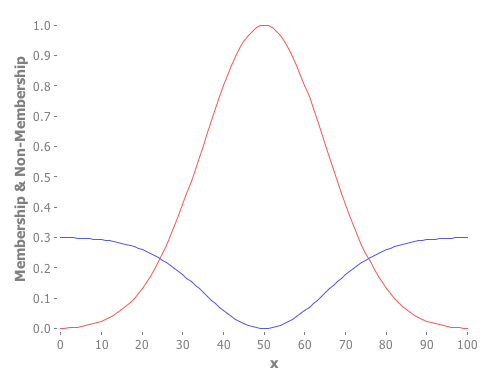
\includegraphics[width=2.5in]{ifs}
  \caption{An Example of an Intuitionistic Fuzzy Set}
  \label{ifs}
\end{figure}

\begin{figure}[!t]
  \centering
  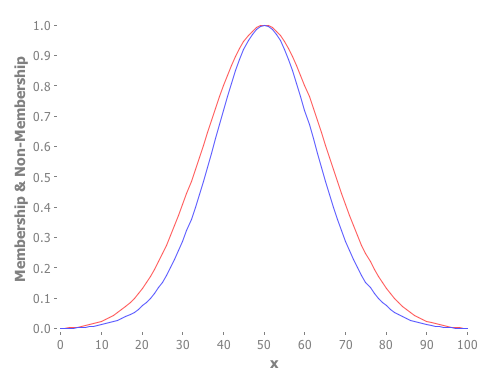
\includegraphics[width=2.5in]{if-membership}
  \caption{Comparison of $\mu(x)$ Against $i\mu(x)$}
  \label{if-membership}
\end{figure}

\begin{figure}[!t]
  \centering
  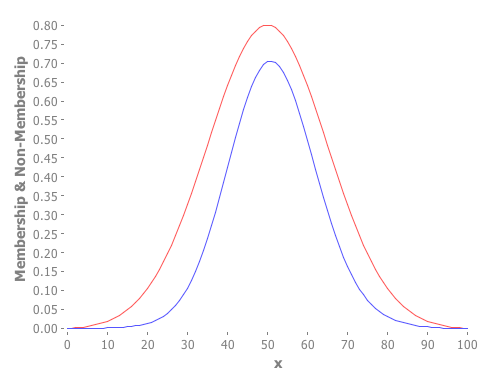
\includegraphics[width=2.5in]{if-membership-drastic}
  \caption{Comparison of $\mu(x)$ Against $i\mu(x)$ With More Indeterminism}
  \label{if-membership-drastic}
\end{figure}

\begin{figure}[!t]
  \centering
  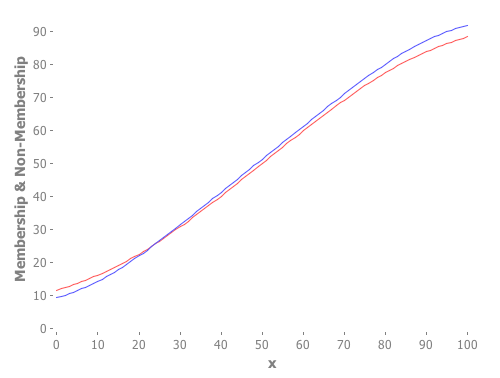
\includegraphics[width=2.5in]{if-coa-vs-coa}
  \caption{Comparison of $CoA(A_{i})$ Against $iCoA{A_{i}}$}
  \label{if-coa-vs-coa}
\end{figure}

% i-membership
\begin{equation}
  i\mu_{A}(x) = (\nu_{A}(x) + \mu_{A}(x))\mu_{A}(x)
\end{equation}

% CoA
\begin{equation}
  A_{CoA} = \dfrac{\sum_{i=1}^{N} \mu(x_{i})
    x_{i}}{\sum_{i=1}^{N} \mu(x_{i})}
\end{equation}

%iCoA
\begin{equation}
  A_{iCoA} = \dfrac{\sum_{i=1}^{N} (\mu(x_{i}) + \nu(x_{i})) \mu(x_{i})
    x_{i}}{\sum_{i=1}^{N} (\mu(x_{i}) + \nu(x_{i})) \mu(x_{i})}
\end{equation}

\begin{equation}
  A_{iCoA} = \dfrac{\sum_{i=1}^{N} i\mu_{A}(x) x_{i}}{\sum_{i=1}^{N}
    i\mu_{A}(x)}
\end{equation}

\section{Experiments}

% \begin{figure}[!t]
%   \centering
%   \includegraphics[width=2.5in]{myfigure}
%   where an .eps filename suffix will be assumed under latex, 
%   and a .pdf suffix will be assumed for pdflatex; or what has been declared
%   via \DeclareGraphicsExtensions.
%   \caption{Simulation results for the network.}
%   \label{fig_sim}
% \end{figure}

\section{Results}

\begin{table}[!t]
  \renewcommand{\arraystretch}{1.3}
  \caption{Hypothesis Tests for the Training Stage}
  \label{hypothesis-tests-training}
  \centering
  \begin{tabular}{|c|c|c|c|c|c|}
    \hline
    Method & $\mu_{TR}$ & $SD_{TR}$ & $n$ & t-Value\\
    \hline
    T1 iFIS & 89.50 & 25.36 & 60 & \\
    \hline
    T1 FIS & 108.05 & 23.47 & 60 & -4.1584 \\
    \hline
    IT2 FIS (\(\mu\)) & 112.56 & 29.16 & 100 & -5.2597 \\
    \hline
    IT2 FIS (SD) & 102.31 & 26.08 & 300 & -3.5548 \\
    \hline
  \end{tabular}
\end{table}

\begin{table}[!t]
  \renewcommand{\arraystretch}{1.3}
  \caption{Hypothesis Tests for the Testing Stage}
  \label{hypothesis-tests}
  \centering
  \begin{tabular}{|c|c|c|c|c|c|}
    \hline
    Method & $\mu_{TS}$ & $SD_{TS}$ & $n$ & t-Value\\
    \hline
    T1-iFIS & 160.99 & 65.70 & 60 & \\
    \hline
    T1-FIS & 194.97 & 71.97 & 60 & -2.7010 \\
    \hline
    IT2-FIS (\(\mu\)) & 192.31 & 105.75 & 100 & -2.3104 \\
    \hline
    IT2-FIS (SD) & 178.63 & 99.70 & 300 & -1.7209 \\
    \hline
  \end{tabular}
\end{table}

% An example of a floating figure using the graphicx package.
% Note that \label must occur AFTER (or within) \caption.
% For figures, \caption should occur after the \includegraphics.
% Note that IEEEtran v1.7 and later has special internal code that
% is designed to preserve the operation of \label within \caption
% even when the captionsoff option is in effect. However, because
% of issues like this, it may be the safest practice to put all your
% \label just after \caption rather than within \caption{}.
% 
% Reminder: the "draftcls" or "draftclsnofoot", not "draft", class
% option should be used if it is desired that the figures are to be
% displayed while in draft mode.
% 
% \begin{figure}[!t]
%   \centering
%   \includegraphics[width=2.5in]{myfigure}
%   where an .eps filename suffix will be assumed under latex, 
%   and a .pdf suffix will be assumed for pdflatex; or what has been declared
%   via \DeclareGraphicsExtensions.
%   \caption{Simulation results for the network.}
%   \label{fig_sim}
% \end{figure}


% An example of a floating table. Note that, for IEEE style tables, the
% \caption command should come BEFORE the table and, given that table
% captions serve much like titles, are usually capitalized except for words
% such as a, an, and, as, at, but, by, for, in, nor, of, on, or, the, to
% and up, which are usually not capitalized unless they are the first or
% last word of the caption. Table text will default to \footnotesize as
% the IEEE normally uses this smaller font for tables.
% The \label must come after \caption as always.
% 
% \begin{table}[!t]
%%   increase table row spacing, adjust to taste
%   \renewcommand{\arraystretch}{1.3}
%   if using array.sty, it might be a good idea to tweak the value of
%   \extrarowheight as needed to properly center the text within the cells
%   \caption{An Example of a Table}
%   \label{table_example}
%   \centering



\section{Conclusion}

\section{Future Work}

\section{Throwing References}

\cite{atanassov1986intuitionistic}
\cite{atanassov2003intuitionistic}
\cite{davarzani2013novel}
\cite{despi2013generalised}
\cite{sharma2011cut}
\cite{sharma2011cutgroups}
\cite{akram2014intuitionistic}
\cite{cornelis2001compositional}
\cite{castillo2007intuitionistic}
\cite{bustince1995method}
\cite{marinov2005method}
\cite{atanassov2013intuitionistic}
\cite{zadeh1965fuzzy}
\cite{klir1995fuzzy}
\cite{pedrycz1998shadowed}
\cite{mendel2001uncertain}
\cite{mendel2002type}
\cite{liang2000interval}
\cite{mendel2006interval}
\cite{karnik2001centroid}
\cite{castro2007interval}
\cite{wagner2013juzzy}

\bibliographystyle{IEEEtran}
\bibliography{paper}

\end{document}
